\chapter{Informe previo}

\section{Rectificador trifásico en estrella con carga R}

Un rectificador trifásico en estrella (Y) es una topología en la cual cada una de las fases comparte una terminal generando el punto neutro y que sirve de referencia para la medición el retorno de cada fase al pasar mediante la carga, esta configuración se puede considerar estandar debido a su amplio uso para la conversión de energía AC trifásica a DC incrementando el voltaje de salida y eficiencia obtenida en comparación a los fuentes monofásicas, un ejemplo de este tipo de rectificador se puede apreciar en la figura \ref{fig:rectificador3-media-onda}

\begin{figure}[h]
	\centering
	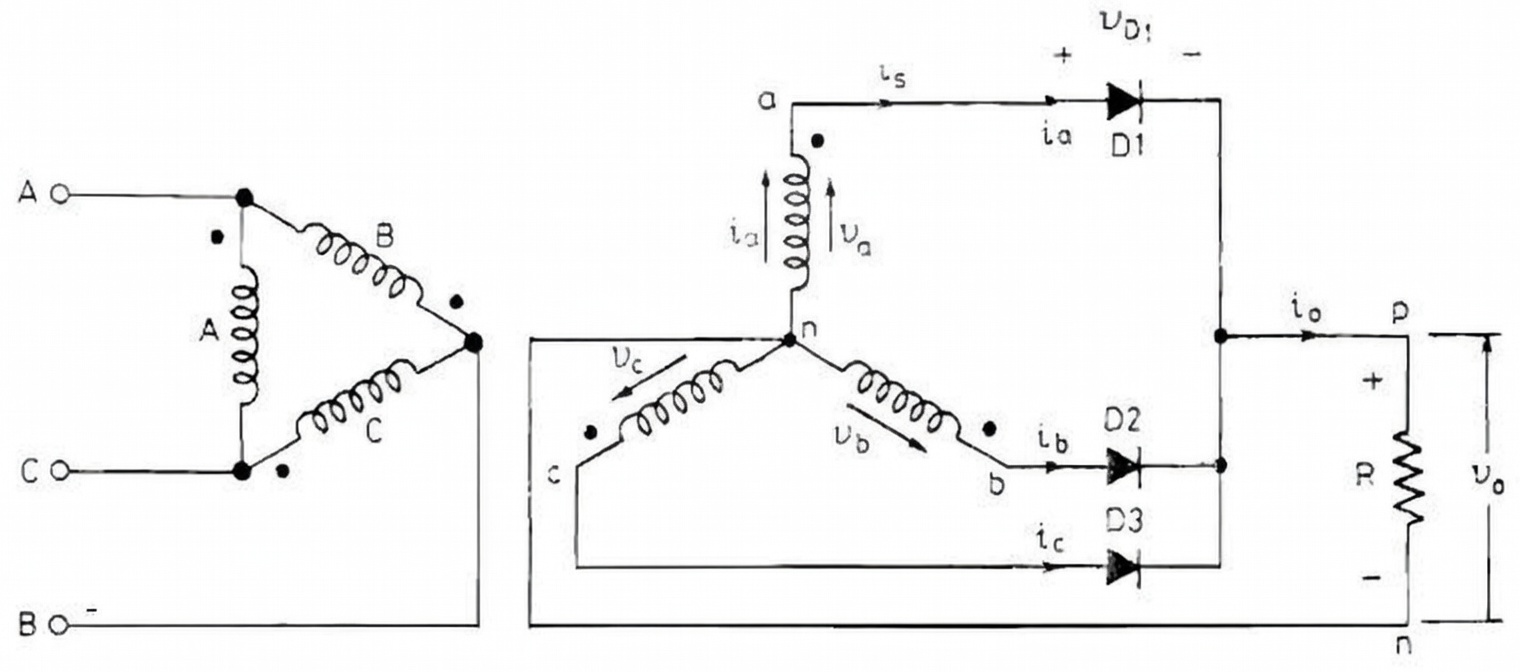
\includegraphics[width=0.8\linewidth]{media/rectificador3-media-onda}
	\caption{Rectificador Trifásico a media onda - Carga R}
	\label{fig:rectificador3-media-onda}
\end{figure}

Y entre sus partes principales podemos encontrar:

\begin{itemize}
	\item Una fuente trifásica balanceada (fases abc).
	\item Tres diodos (rectificador de media onda trifásico).
	\item La carga conectada entre el neutro del sistema y la salida común de los diodos.
\end{itemize}

Cada diodo conduce cuando su tensión de fase es la más positiva respecto al neutro como se muestra en la figura \ref{fig:fases-conduccion-3p} considerando para esto un sistema ideal balanceado para una conducción por diodo de 120°, generando una salida formada por tres semiciclos positivos desplazados 120°, lo que produce una tensión pulsante DC con frecuencia de rizado $3f$.

\begin{figure}[h]
	\centering
	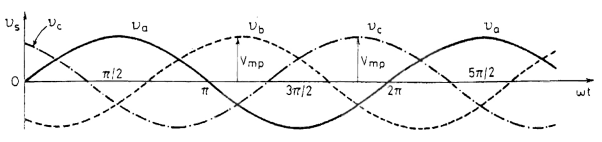
\includegraphics[width=0.7\linewidth]{media/fases-conduccion-3p}
	\caption{Fases de conducción - Rectificador trífasico a media onda}
	\label{fig:fases-conduccion-3p}
\end{figure}

\section{Tipos de carga en los rectificadores Trifásicos}

\subsection{Rectificador trifásico en estrella con carga RC}

Al agregar un capacitor en paralelo con la carga R, el capacitor se carga hasta el máximo de la tensión rectificada y se descarga lentamente a través de la resistencia cuando los diodos dejan de conducir. El resultado de este proceso es:

\begin{itemize}
	\item Incremento del valor medio DC
	\item Reducción significativa del rizado
	\item Corrientes de diodo no sinusoidales y pulsantes
	\item Mayor corriente pico en los diodos y el transformador
\end{itemize}

Este comportamiento agregar cierto estrés térmico a los diodos y el transformador a causa del incremento del voltaje agregado en la descarga del capacitor, por lo que debe ser considerado en el diseño para mitigar tales efectos mediante disipadores o componentes más robustos.

Finalmente se muestra una tabla comparativa \ref{tab:carga-R-RC} entre un rectificador trifásico en estrella con carga R y RC. 

\begin{table}[htbp]
	\centering
	\begin{tabular}{lcc}
		\toprule
		Característica & Carga R & Carga RC \\
		\midrule
		Forma de onda & Pulsante trifásica & Cuasi continua \\
		Rizado & Alto & Bajo \\
		Corriente del diodo & Suave & Pulsante \\
		Valor DC & Menor & Mayor \\
		Factor de potencia & Mejor & Peor \\
		Estrés en diodos & Menor & Mayor \\
		\bottomrule
	\end{tabular}
	\caption{Tabla comparativa carga R/RC - Rectificador trifásico a media onda}
	\label{tab:carga-R-RC}
\end{table}

\section{Parámetros del rectificador trifásico}

Para comprender el funcionamiento de este tipo de rectificador es necesario realizar el análisis físico (composición), eléctrico (variación señales) y finalmente el matemático para la obtención de expresiones matemáticas o relaciones que permitan validar los valores obtenidos experimentalmente.

Por tanto se tiene que: \\

\subsection*{(a) Voltaje pico $V_m$}
Para un sistema trifásico balanceado:
\[
V_m = \sqrt{2} \, V_{\text{fase,rms}}
\]

Si se parte de tensión línea--línea:
\[
V_{\text{fase,rms}} = \frac{V_{LL}}{\sqrt{3}}
\]

\subsection*{(b) Voltaje medio $V_{\text{medio}}$ (DC)}
Para rectificador trifásico de media onda:
\[
V_{\text{medio}} = \frac{3\sqrt{3}}{2\pi} V_m \approx 0.827V_m
\]
Este valor aumenta al agregar capacitor.

\subsection*{(c) Voltaje eficaz $V_{\text{rms}}$}
Para carga resistiva:
\[
V_{\text{rms}} = V_m \sqrt{\frac{3}{2\pi} \int_{\pi/6}^{5\pi/6} \sin^2(\theta) \, d\theta}
\]

Resultado típico:
\[
V_{\text{rms}} \approx 0.84V_m
\]

\subsection*{(d) Corriente media $I_{\text{media}}$}
\[
I_{\text{media}} = \frac{V_{\text{medio}}}{R}
\]

\subsection*{(e) Corriente eficaz $I_{\text{rms}}$}
\[
I_{\text{rms}} = \frac{V_{\text{rms}}}{R}
\]

\subsection*{(f) Rizado $r$}
\[
r = \sqrt{\left(\frac{V_{\text{rms}}}{V_{\text{medio}}}\right)^2 - 1}
\]

Carga R típica:
\[
r \approx 0.18
\]

Carga RC:
\[
r \ll 0.1
\]

\subsection*{(g) Potencia AC $P_{\text{ac}}$}
\[
P_{\text{ac}} = 3 \, V_{\text{fase,rms}} \, I_{\text{fase,rms}}
\]

\subsection*{(h) Potencia DC $P_{\text{dc}}$}
\[
P_{\text{dc}} = V_{\text{medio}} \cdot I_{\text{media}}
\]

\subsection*{(i) Rendimiento $\eta$}
\[
\eta = \frac{P_{\text{dc}}}{P_{\text{ac}}}
\]

\subsection*{(j) Factor de forma $FF$}
\[
FF = \frac{V_{\text{rms}}}{V_{\text{medio}}}
\]

\subsection*{(k) Factor de rizado $RF$}
\begin{align*}
	RF &= \frac{V_{\text{ac,rms}}}{V_{\text{dc}}} \\
	&= \sqrt{FF^2 - 1}
\end{align*}

\subsection*{(l) Factor de utilización del transformador (TUF)}
\[
TUF = \frac{P_{\text{dc}}}{3V_{\text{fase,rms}} I_{\text{fase,rms}}}
\]

Valor típico:
\[
TUF \approx 0.69
\]

\subsection*{(m) Factor de potencia $FP$}
\[
FP = \frac{P_{\text{ac}}}{S} = \frac{P_{\text{ac}}}{3V_{\text{fase,rms}} I_{\text{fase,rms}}}
\]

Con carga RC: Distorsión armónica $\rightarrow$ FP bajo.

\subsection*{(n) Voltaje pico inverso del diodo (PIV)}
\[
PIV = 2V_m
\]

Este valor debe ser considerado con margen de seguridad $\geq 30\%$.

\subsection*{(o) Corriente pico del diodo $I_p$}
Para carga R:
\[
I_p = \frac{V_m}{R}
\]

Para carga RC:
\[
I_p \gg \frac{V_m}{R}
\]
(dependiente de $C$ y resistencia equivalente)

\subsection*{(p) Frecuencia de la onda rectificada $f_r$}
\[
f_r = 3f
\]

\section{Formas de onda del rectificador}

Una forma de poder comprender el funcionamiento de este tipo de rectificadores es mediante el empleo de las formas de onda que permiten visualizar exactamente cuándo y por cuánto tiempo conduce cada diodo. En un rectificador trifásico, la conducción no es continua ni simultánea, sino que se reparte en intervalos angulares definidos (por ejemplo, 120°). Sin la gráfica, este fenómeno queda oculto en las ecuaciones promedio, pero en laboratorio se manifiesta claramente como segmentos de tensión y corriente activos e inactivos. Esto es clave para entender el reparto de corrientes, el calentamiento de los semiconductores y el funcionamiento correcto de la topología.


\begin{figure}[h]
	\centering
	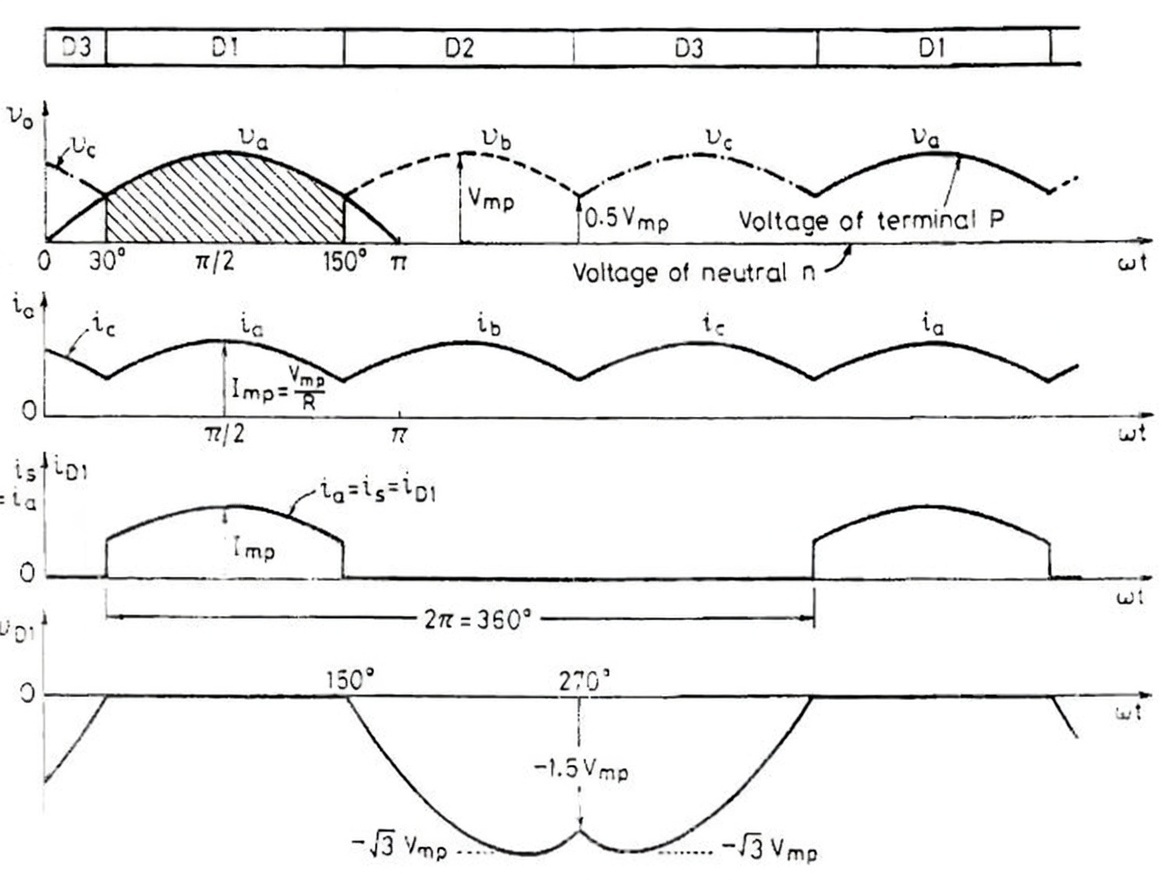
\includegraphics[width=0.8\linewidth]{media/formas-onda-rect-3p}
	\caption{Formas de onda del rectificador trifásico a media onda}
	\label{fig:formas-onda-rect-3p}
\end{figure}

En la figura \ref{fig:formas-onda-rect-3p} se muestran las formas de onda del rectificador trifásico a media onda con conexión en estrella y carga resistiva, y representan de manera directa el proceso físico a nivel de señales de lo que ocurre en el circuito rectificador comprobando así que en cada fase de la fuente trifásica alimenta un diodo, y la salida se toma respecto al neutro.

Las tensiones de fase senoidales se representan como $v_a$, $v_b$ y $v_c$ estando estas equilibradas y desfasadas $120^\circ$ respecto a la otra, logrando así que la tensión de salida $v_o$ rectificada resulta de seleccionar en cada instante el mayor valor positivo entre estas tres tensiones, por lo que su forma de onda corresponde a la envolvente superior de las tensiones de fase y en donde cada diodo conduce durante un intervalo de $120^\circ$ equivalente con el periodo o tiempo de en el cual cada señal es mayor a las otras.

Finalmente en la figura \ref{fig:formas-onda-rect-3p} también se puede destacar las formas de onda de las tensiones inversa aplicada a un diodo cuando este no conduce en su estado de polarización en inversa por la diferencia entre las tensiones de fase, alcanzando valores negativos elevados. El valor máximo de esta tensión inversa, conocido como voltaje pico inverso, es del orden de $\sqrt{3}V_{mp}$, y en ciertos instantes puede aproximarse a valores cercanos a $-1.5V_{mp}$. Esta información es crítica para el dimensionamiento correcto de los diodos, ya que define el nivel mínimo de tensión inversa que deben soportar con un margen de seguridad adecuado para que no se tengan un mal funcionamiento de los mismos logrando afectar al comportamiento general del circuito.